\documentclass{beamer}

%\usepackage{beamerthemesidebar, fancybox}
\usepackage{beamerthemesplit,fancybox}
%\usepackage[pdftex]{color,graphicx}
\usepackage{graphicx,pgfarrows,pgfnodes}
%\usepackage{pgfarrows,pgfnodes}
\usepackage{verbatim} % for block comments, so I can comment out entire slides easily

%\usepackage{pgfpages}
%\pgfpagesuselayout{resize}[a4paper,border shrink=5mm,landscape]

\usepackage{mjclectureslides}


\definecolor{Dblue}{rgb}{.255,.41,.884}

\title[Linear Algebra Preliminaries: set notation, dimension]{Linear Algebra and Matrix Methods \\ Introduction to set notation, dimension}
%\author[Prof. Michael Carlisle]{Prof. Michael Carlisle}
%\institute{Baruch College, CUNY}
%\date{Spring 2018}
\date{}
% 

\begin{document}

\frame{\titlepage}


\frame{ \frametitle{Introduction}

\begin{center}
The point of this course is to understand, 

\vspace{5mm}

and understand how to solve, 

\vspace{5mm}

systems of linear equations.
\end{center}

}


\frame{ \frametitle{Set / Element}

To understand the language of linear algebra, we start with the basic definitions of set notation.

\vspace{5mm}

\begin{defn} A \textbf{set} is a collection of distinct objects, called the set's \textbf{elements}. 

\vspace{5mm}

The elements:
\begin{itemize}
\item do not necessarily have an inherent order or relationship to each other (although they usually will); 
\item duplicates are not allowed; 
\item they are merely \emph{different things in the same bag}. 
\end{itemize}
\end{defn}

}


\frame{ \frametitle{Set / Element Notation}

``The set $A$ contains three elements: 

\begin{center}
`cat', `tree', and the number 6.''
\end{center}

This is denoted 
\[ A = \{ \text{tree}, \text{cat}, 6 \} \]

\vspace{3mm}

with curly brackets indicating the set.

\vspace{5mm}

This is an \emph{explicit} definition of a particular set. It has 3 elements.

\vspace{5mm}

``6 is an element of $A$'' is denoted $6 \in A$.\\

\vspace{5mm}

``'dog' is not an element of $A$'' is denoted dog $\not \in A$. 

}



\frame{ \frametitle{Set / Element Notation}

``The set $B$ consists of the even numbers \emph{strictly} between 0 and 25'' 
(i.e. \emph{exclusive}) is an \emph{implicit} definition of the set denoted 

\vspace{3mm}

\[ B = \{ 2, 4, 6, ..., 22, 24\}. \]

\vspace{5mm}

The \emph{ellipsis} ``...'' means: 

\begin{center}
``you understand the pattern given by the context''.
\end{center}

}


\frame{ \frametitle{Set / Element Notation}

Another way to write

\vspace{3mm}

\[ B = \{ 2, 4, 6, ..., 22, 24\} \]

\vspace{3mm}

is 

\vspace{3mm}

\[ B = \{ x \in \mathbb{Z} \, | \, 0 < x < 25, \, x \text{ even}\}, \]

\vspace{3mm}

where the vertical bar $|$ means ``such that''. 

\vspace{3mm}

(Sometimes a colon : is used instead of the bar $|$.)

}



\frame{ \frametitle{Popular Number Sets}

$\mathbb{N} = \{ 1, 2, 3, ... \}$ is the set of \textbf{natural numbers} \\
or \textbf{counting numbers} (and sometimes contains 0). 

\vspace{10mm}

$\mathbb{Z} = \{ ..., -3, -2, -1, 0, 1, 2, 3, ... \}$ is the set of \textbf{integers} \\
(written with a Z for the German word Zahlen (``numbers'')). 

\vspace{10mm}

 $\mathbb{Q} = \{ \frac{m}{n} \, | \, m, n \in \mathbb{Z}, \, n \neq 0 \}$ is the set of \textbf{rational numbers} \\
 (i.e. fractions, ratios; the Q stands for ``quotient''). 

}


\frame{ \frametitle{Real Number Sets}

$\mathbb{R}$ is the set of \textbf{real numbers}, containing all rational and irrational numbers. This is the set of numbers along the continuous number line, containing all infinite-length decimal expansions. 

\vspace{4mm}

\begin{figure}[!ht]
  \centering
    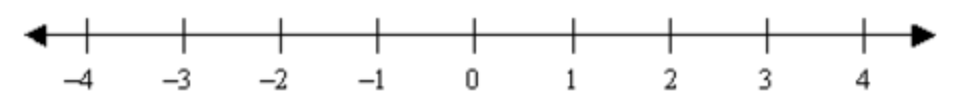
\includegraphics[width=4in]{numberline.png}
\end{figure}

\vspace{4mm}

An \textbf{open interval} of real numbers is denoted 

\[ (a, b) = \{ x \in \mathbb{R} : a < x < b \}. \]

A \textbf{closed interval} of real numbers is denoted 

\[ [a, b] = \{ x \in \mathbb{R} : a \leq x \leq b \}. \]

}



\frame{ \frametitle{Empty Set}

The \textbf{empty set} is the set with no elements (think: an empty bag). 

\vspace{5mm}

It is denoted 

\[ \emptyset \] 

and defined with curly brackets by 

\[ \emptyset = \{\}. \]

}


\frame{ \frametitle{Union}

Some basic operations we can use on sets are: 

\vspace{5mm}

The \textbf{union} of the sets $A$ and $B$ is the set of all elements of $A$ and $B$ combined. It is denoted $A \cup B$, and defined by 

\[ A \cup B = \{ x : \, x \in A \text{ or } x \in B \text{ (or both)}\}. \]

\begin{figure}[!ht]
  \centering
    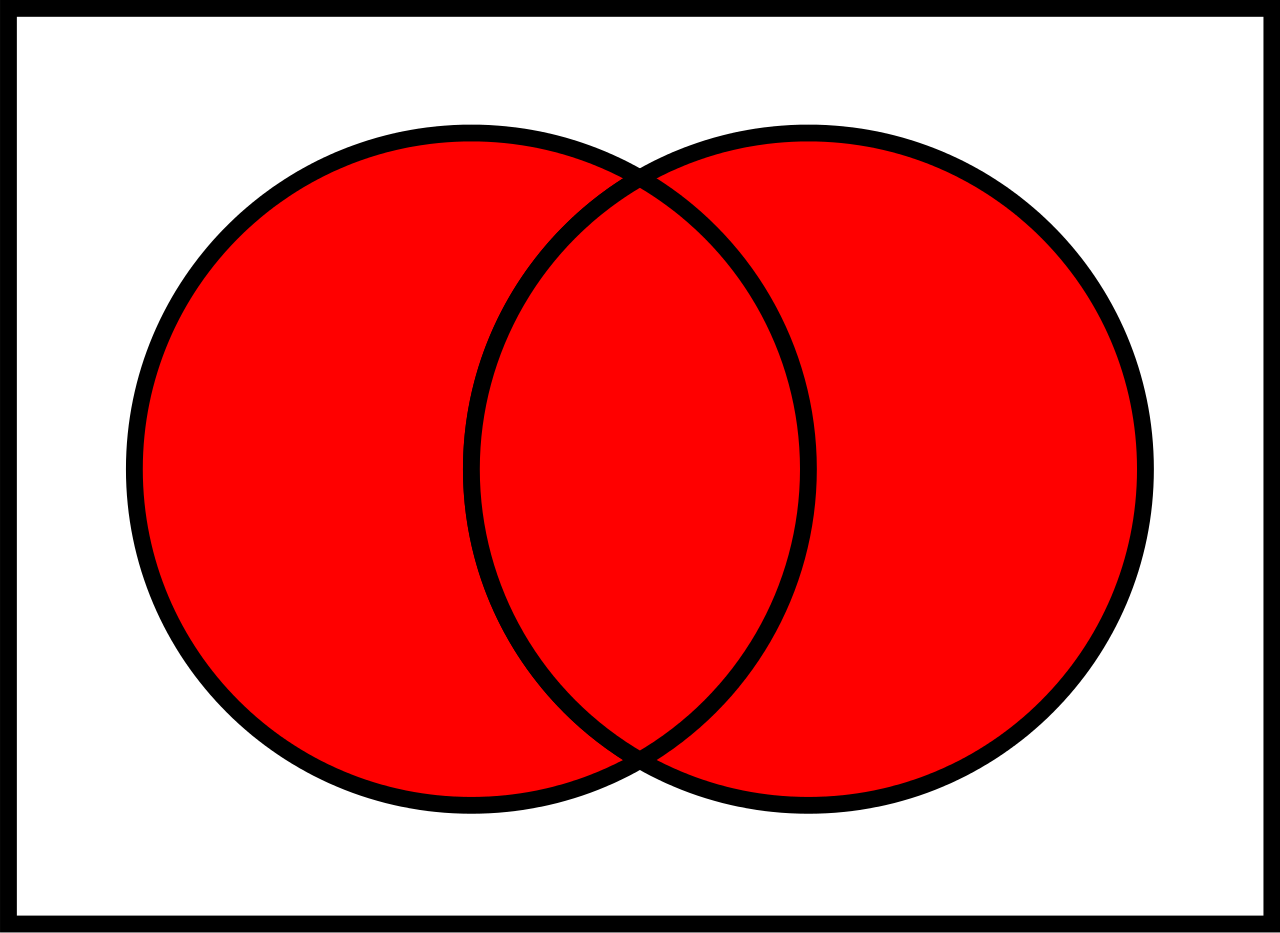
\includegraphics[width=2in]{union.png}
\end{figure}


}


\frame{ \frametitle{Intersection}

The \textbf{intersection} of the sets $A$ and $B$ is the shared elements of $A$ and $B$. It is denoted $A \cap B$ or $AB$, and defined by 

\[ A \cap B = \{ x : \, x \in A \text{ and } x \in B \}. \]

\begin{figure}[!ht]
  \centering
    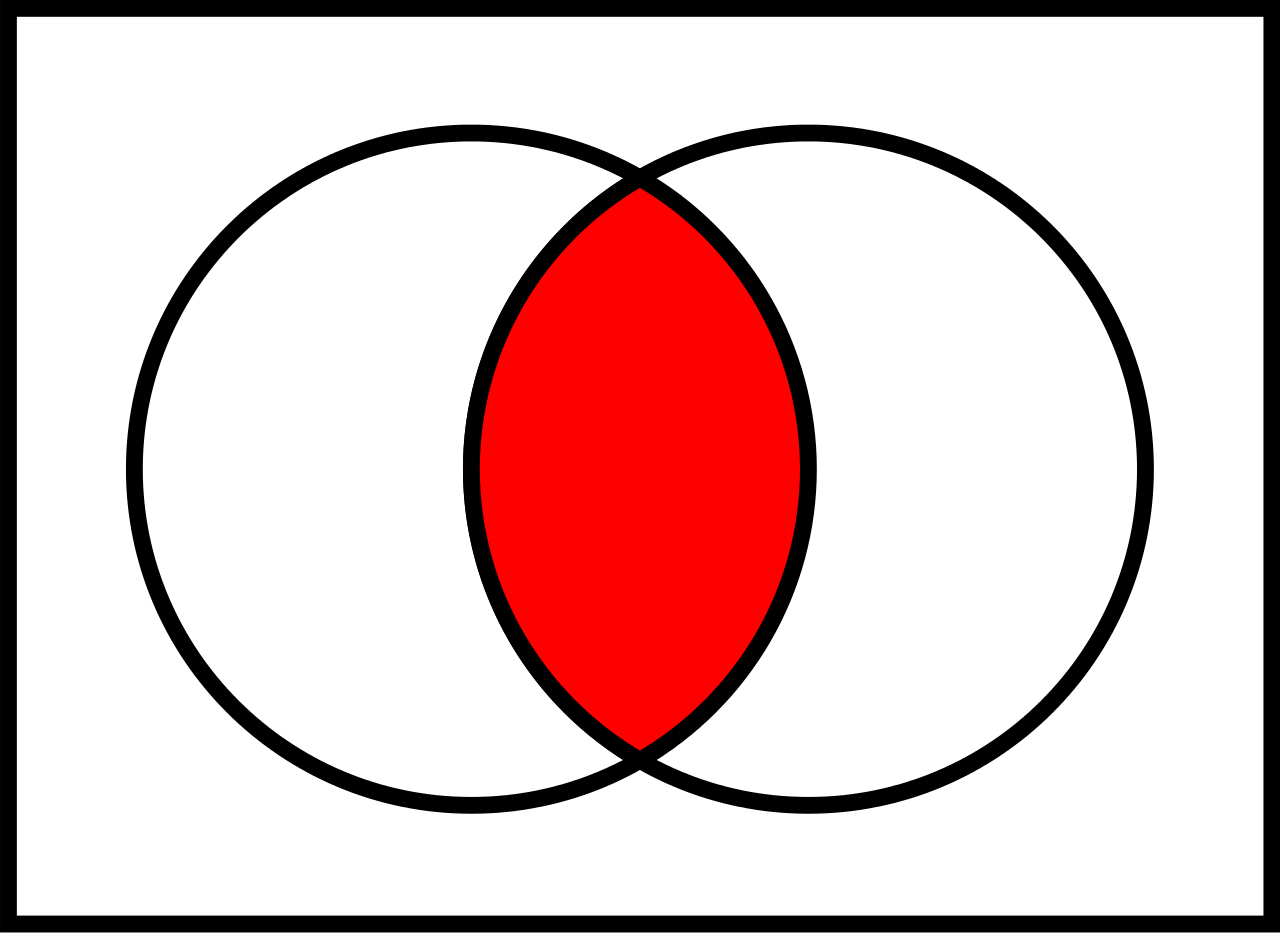
\includegraphics[width=2in]{intersection.png}
\end{figure}

If $A$ and $B$ have no common elements, we say $A$ and $B$ are \textbf{disjoint} sets and denote this fact by  $A \cap B = \emptyset$.

}



\frame{ \frametitle{Set Difference}

The \textbf{set difference} $B \setminus A$ (sometimes denoted $B - A$) is the elements of $B$ with the shared elements of $A$ removed. It is denoted 
\[ B \setminus A = \{ x : \, x \in B \text{ and } x \not \in A \}. \]

\begin{figure}[!ht]
  \centering
    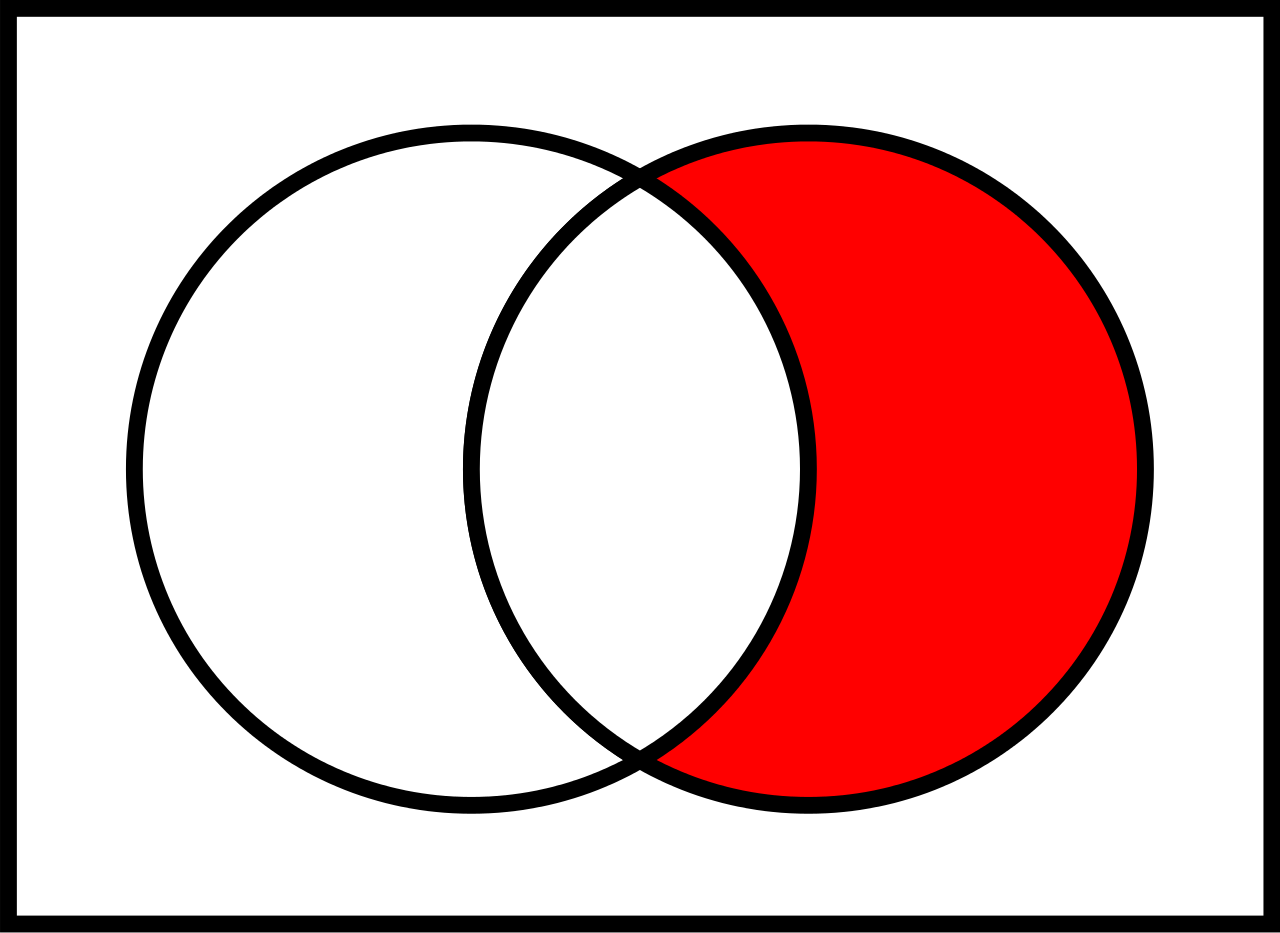
\includegraphics[width=2in]{BminusA.png}
\end{figure}

}


\frame{ \frametitle{Set Difference}

\[ A = \{ 1, 2, 5, 6, 7\}, \,\,\, B = \{ 2, 5, 8, 9, 13\} \]

\[ \implies A \setminus B = \{ 1, 6, 7\} \text{ but } B \setminus A = \{8, 9, 13\}. \]

\begin{figure}[!ht]
  \centering
    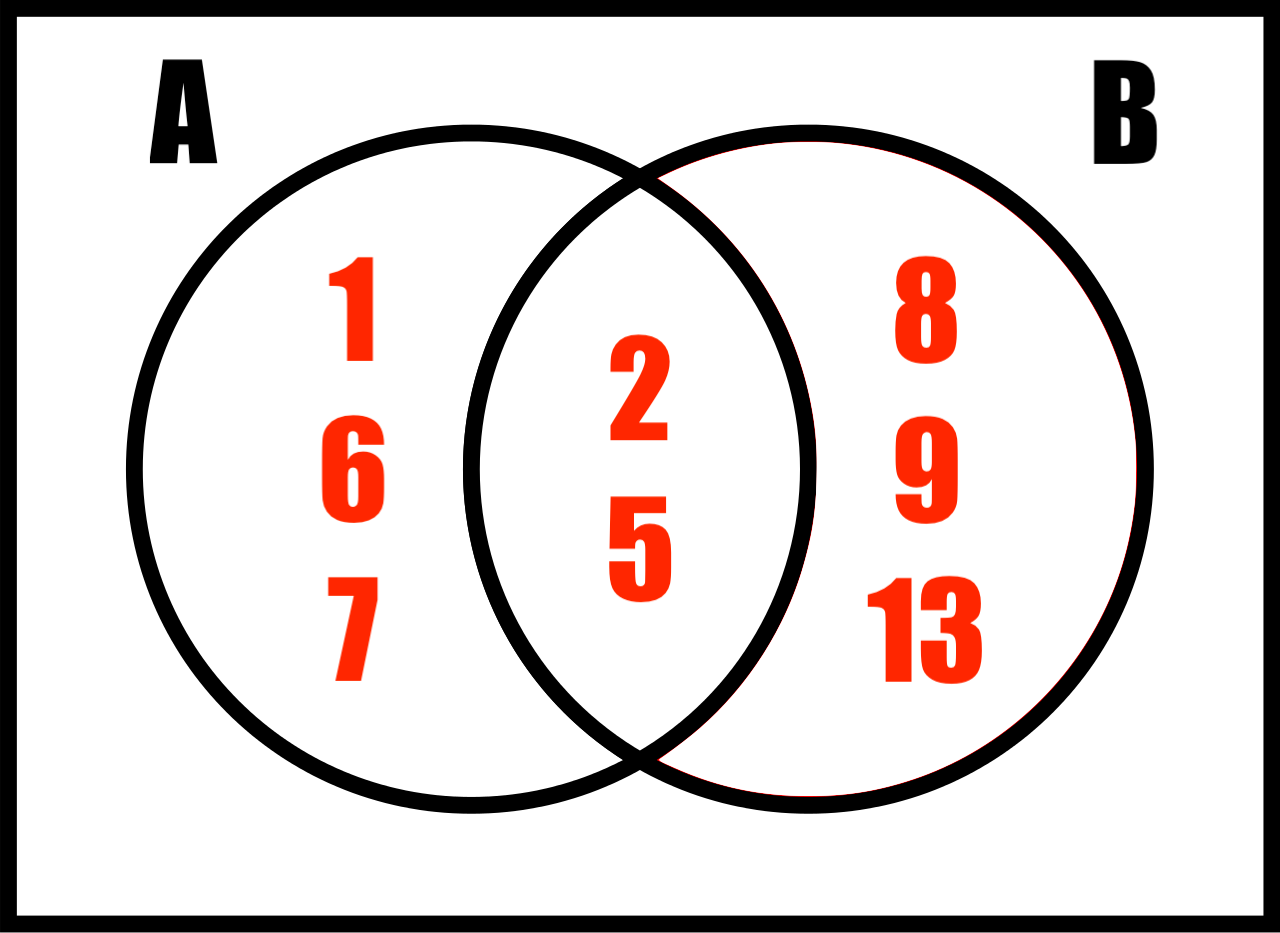
\includegraphics[width=2in]{BminusAexample.png}
\end{figure}

\begin{center}
Thus, $A \setminus B \neq B \setminus A$ (an important general result). 
\end{center}

}


\frame{ \frametitle{Subset}

The set $A$ is called a \textbf{subset} of $B$, denoted $A \subseteq B$, if all of $A$'s elements are in $B$. 
\[ A \subseteq B \iff (x \in A \implies x \in B). \]
\begin{figure}[!ht]
  \centering
    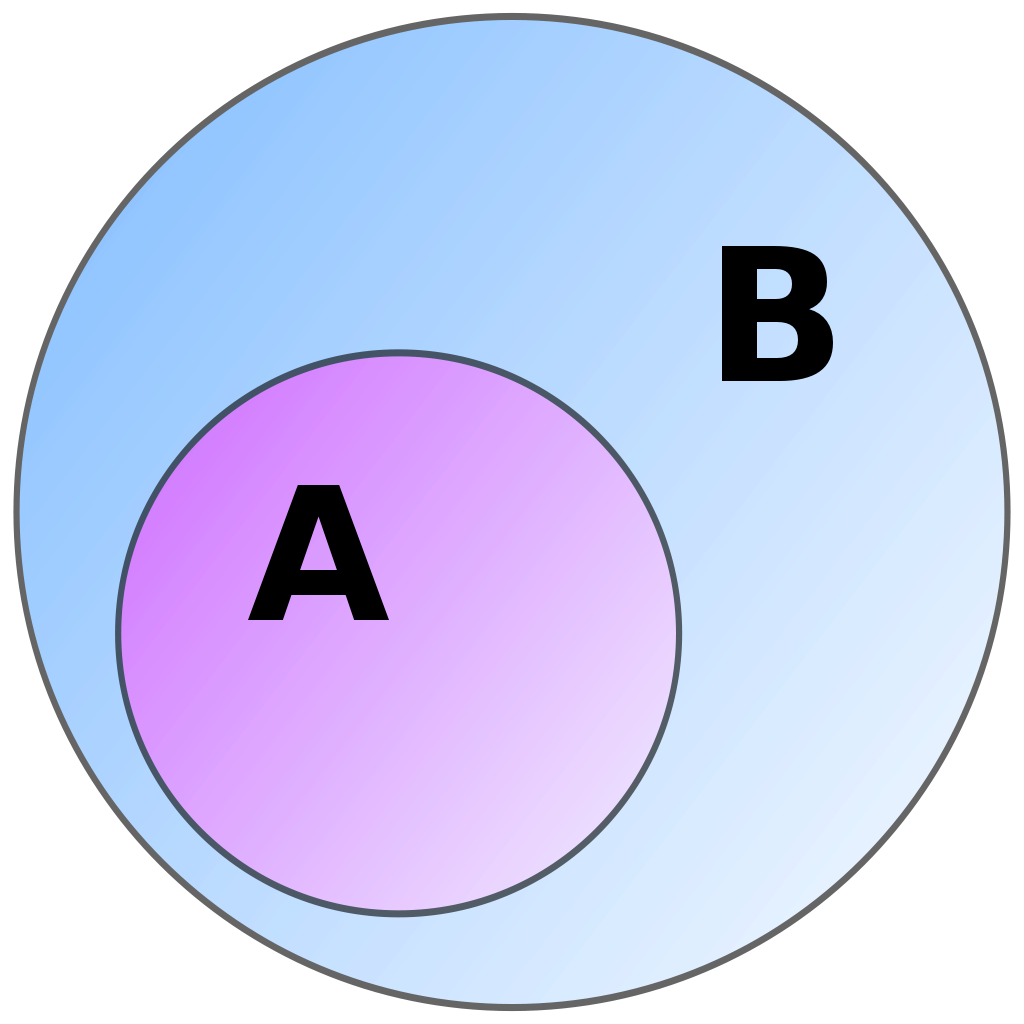
\includegraphics[width=2in]{AsubsetB.png}
\end{figure}

Two sets $A$ and $B$ are \textbf{equal} (written $A = B$) if $A \subseteq B$ and $B \subseteq A$.

}


\frame{ \frametitle{Universal Set, Complement}

In certain collections of problems, we may define a \textbf{universal set} as a common ``top-level set'' under which all the sets described in the problem are subsets of. 

\begin{figure}[!ht]
  \centering
    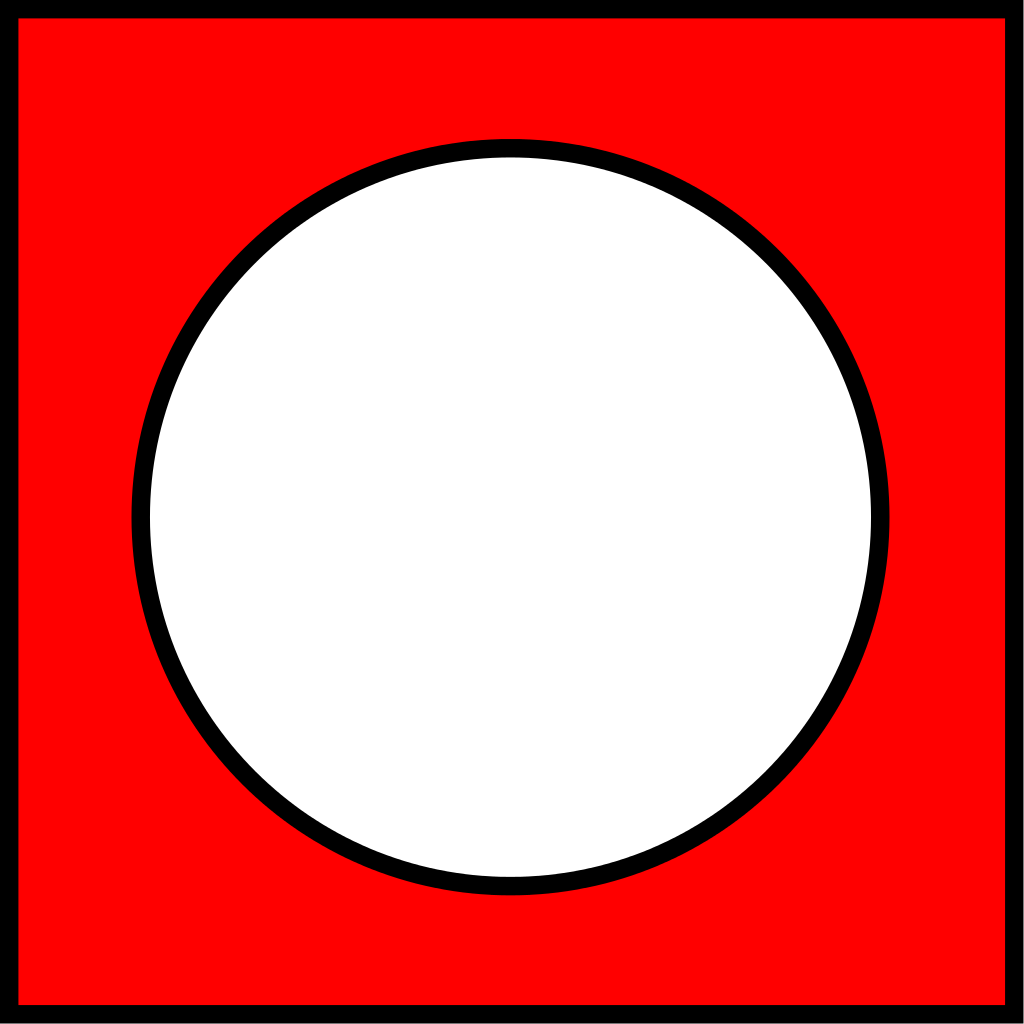
\includegraphics[width=2in]{Acomplement.png}
\end{figure}

}


\frame{ \frametitle{Universal Set, Complement}

The \textbf{complement} of a set $A$, relative to the universal set $U$, is denoted $A^C = U \setminus A$. (Some texts use $A'$ or $\overline{A}$.)

\begin{figure}[!ht]
  \centering
    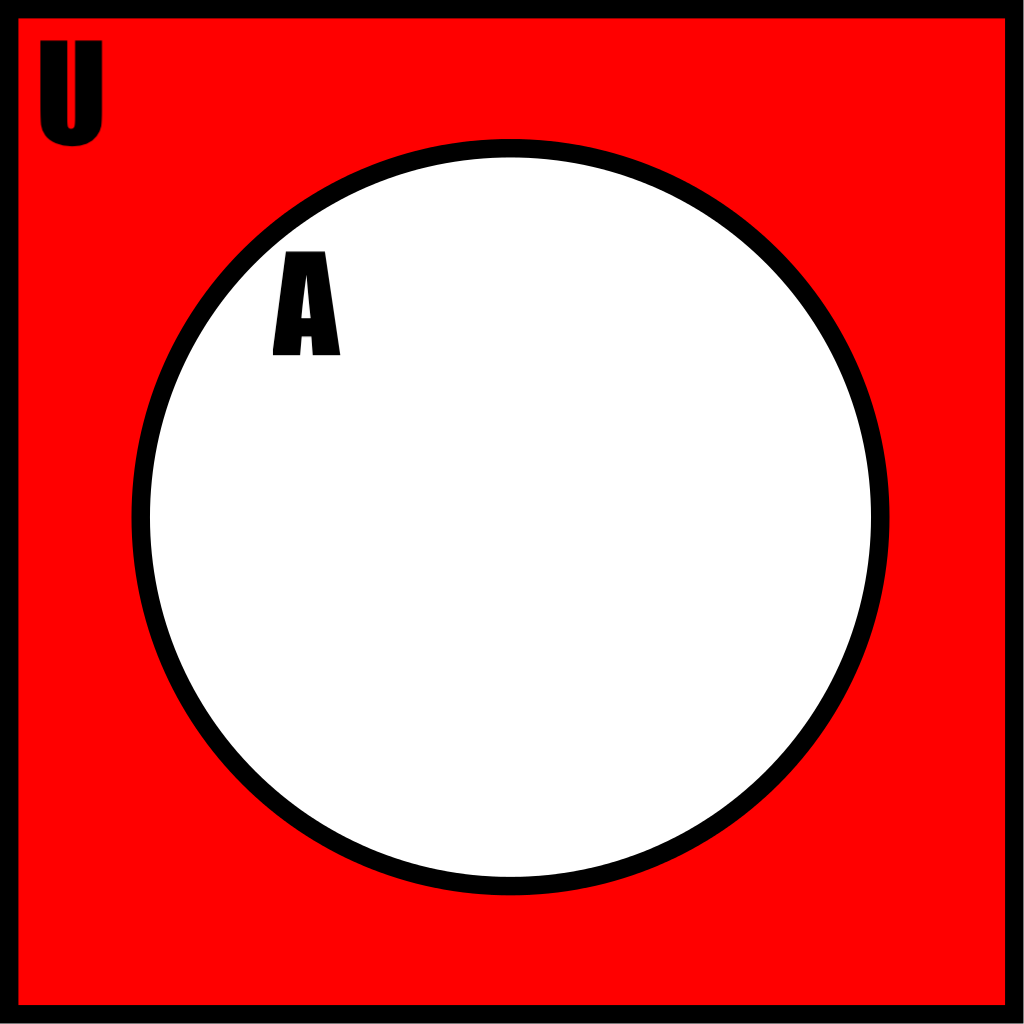
\includegraphics[width=2in]{Acomplement2.png}
\end{figure}

Using this, we can define the set difference as $A \setminus B = A \cap B^C$. 

}


\frame{ \frametitle{Example}

Considering $\R$ as the universal set, and let 
\vspace{5mm}
\[ A = (1,\infty) = \{ x \in \R: x > 1\}. \]
\vspace{5mm}
Then 
\vspace{5mm}
\[ A^C = \R \setminus A = (-\infty, 1] = \{ x \in \R: x \leq 1\}. \]

}


\frame{ \frametitle{Unions, Intersections, Complements}

Union and intersection are \emph{commutative} operations: 
\vspace{5mm}
\[ A \cup B = B \cup A, \,\, A \cap B = B \cap A. \]

\vspace{5mm}

We've already seen that set difference is \emph{not} commutative: 

\vspace{5mm}

\[ A \setminus B \neq B \setminus A. \]

}


\frame{ \frametitle{Unions, Intersections, Complements}

Union and intersection are also \emph{associative}: 
\vspace{5mm}
\[ (A \cup B) \cup C = A \cup (B \cup C), \,\, (A \cap B) \cap C = A \cap (B \cap C). \]

\vspace{5mm}

Regardless of universal set, it should be clear that the complement of a complement is the original set: 

\vspace{5mm}

\[ (A^C)^C = A. \]

}



\frame{ \frametitle{Tuples, Dimension}

An \textbf{ordered pair} of real numbers, often written $(x,y)$, is an element of ``the two-dimensional plane'', called $\R^2$:
\[ \R^2 = \{ (x,y): \, x,y \in \R \}. \] 

\vspace{5mm}

An \textbf{ordered triple} of real numbers, often written $(x,y,z)$, is an element of ``three-dimensional space'', called $\R^3$: 
\[ \R^3 = \{ (x,y,z): \, x,y,z \in \R \}. \] 

\vspace{5mm}

In general, an \textbf{ordered $n$-tuple} of real numbers, often written $(x_1, x_2, ..., x_n)$, is an element of ``$n$-dimensional space'', called $\R^n$: 
\[ \R^n = \{ (x_1, x_2, ..., x_n): \, x_1, x_2, ..., x_n \in \R \}. \] 

}


\frame{ \frametitle{Tuples, Dimension}

The number $n$ in this context is called the \textbf{dimension} of the space we are considering. This $n$ describes the number of \textbf{coordinates}, or separate ordered values, in the tuple. \\

\vspace{10mm}

Later, we will see a more general definition of the terms \textbf{space} and \textbf{dimension}, and how they are related.

}



\frame{ \frametitle{Mathematical Space}

A mathematical set with some extra structure on it, like a mathematical operation such as addition or multiplication, is called a \textbf{space}.

\vspace{10mm}

For example, the real numbers $\R = (-\infty, \infty)$ is a set, but the real numbers \emph{with addition} $(\R, +)$ is a space.

}


\frame{ \frametitle{Mathematical Space, Subspace}

A \textbf{subspace} of a space is a subset of a space's set that still lets you use the operation(s) available to the original space. 

\vspace{8mm}

For example, the integers $\Z$ is a subset of $\R$, but the integers \emph{with addition} $(\Z, +)$ is a subspace of $(\R, +)$ because we can still ``do addition'' with just integers. (+ is called ``closed'' under $\Z$.)

\vspace{8mm}

The main objects we will examine in this course are called \textbf{vectors}. They exist in \textbf{vector spaces}.

}


\end{document}
